%\documentclass{beamer}
\documentclass[serif, 11pt]{beamer}

\usepackage{graphicx} % Allows including images
\usepackage{booktabs} % Allows the use of \toprule, \midrule and \bottomrule in tables
\usepackage[utf8]{inputenc}
\usepackage{amsmath}

\graphicspath{{fig/} {../src/fig/}}

\setbeamertemplate{navigation symbols}{}%remove navigation symbols
\setbeamertemplate{footline}[frame number]
\setbeamerfont{page number in head/foot}{size=\normalsize}

\begin{document}

\begin{frame}{Implementation of the simulator}

\begin{itemize}
	\item The Pong is implemented using \texttt{pygame}
	\item Two modes of operation:
	\begin{itemize}
		\item \textbf{Training}: no drawing, only physics (machine speed).
		\item \textbf{Play}: Visually see the trained controller (human speed).
	\end{itemize}
	\item Each controller is trained against a robotic reference controller that 
		only follows the ball.
	\item Same CPU time for all controllers, by default 30 min.
\end{itemize}


\end{frame}


\begin{frame}{Blueprints}
	\begin{center}
		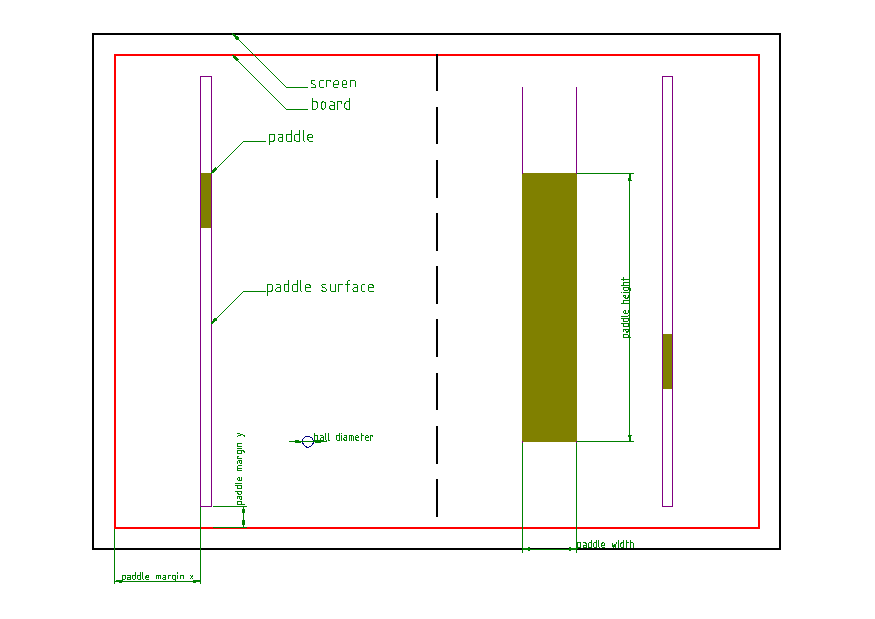
\includegraphics[width=\linewidth]{pong.pdf}
	\end{center}
\end{frame}

\begin{frame}{Pygame implementation}
	\begin{center}
		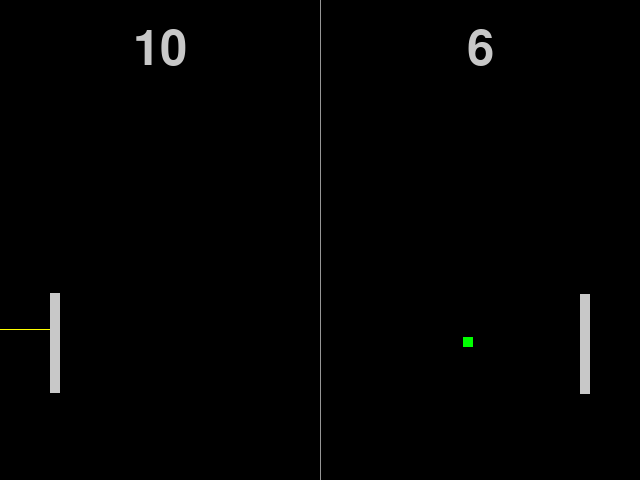
\includegraphics[width=.8\linewidth]{pong-QL3.png}
	\end{center}
\end{frame}

\begin{frame}{State mapping (QL and SARSA)}
	\begin{itemize}
		\item How can we translate the state of the game $\theta = (v_1, v_2, 
			\ldots, v_n)$ (position and velocity of the ball, paddles...) into a 
			single number, the state $0 \le s < N$?
			%
			$$ \theta \xrightarrow{?} s $$

		\item We first \textbf{discretize} all the variables $\tilde \theta$, then 
			we assign a number to the ordered values of $\tilde \theta$.

		\item The number of states $N$ grows \textbf{exponentially} with the number of 
			variables $n$.
	\end{itemize}
\end{frame}

\begin{frame}{Measure of training performance}
	\begin{itemize}
		\item In order to measure how well a controller is playing against the 
			opponent, we use a normalized score $d$. Let $S_C$ be the score of the 
			controller and $S_O$ of the opponent,
			%
			$$ d = 2 \frac{S_C - S_O}{S_C + S_O} $$

		\item The value $d$ is less, equal or bigger than $0$ if the controller 
			behaves worse, similarly or better than the opponent, respectively.
		\item We want to maximize the $d$ value.
	\end{itemize}
\end{frame}

\begin{frame}{Results: 30 min of training}
	\begin{center}
		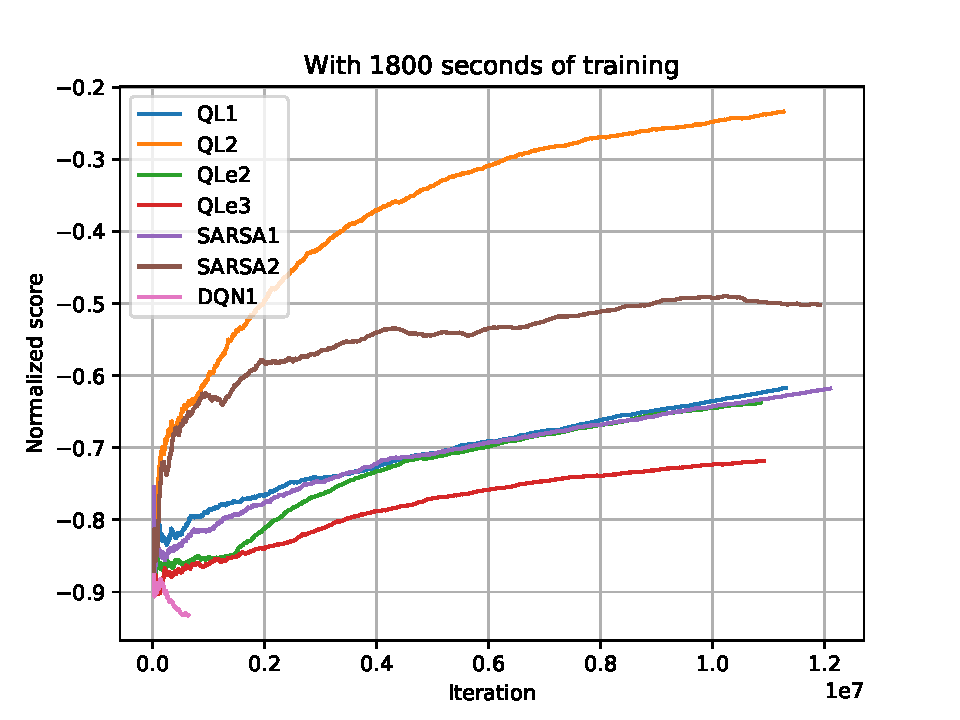
\includegraphics[width=.9\linewidth]{score-1800.pdf}
	\end{center}
\end{frame}

\begin{frame}{Results: 2h of training}
	\begin{center}
		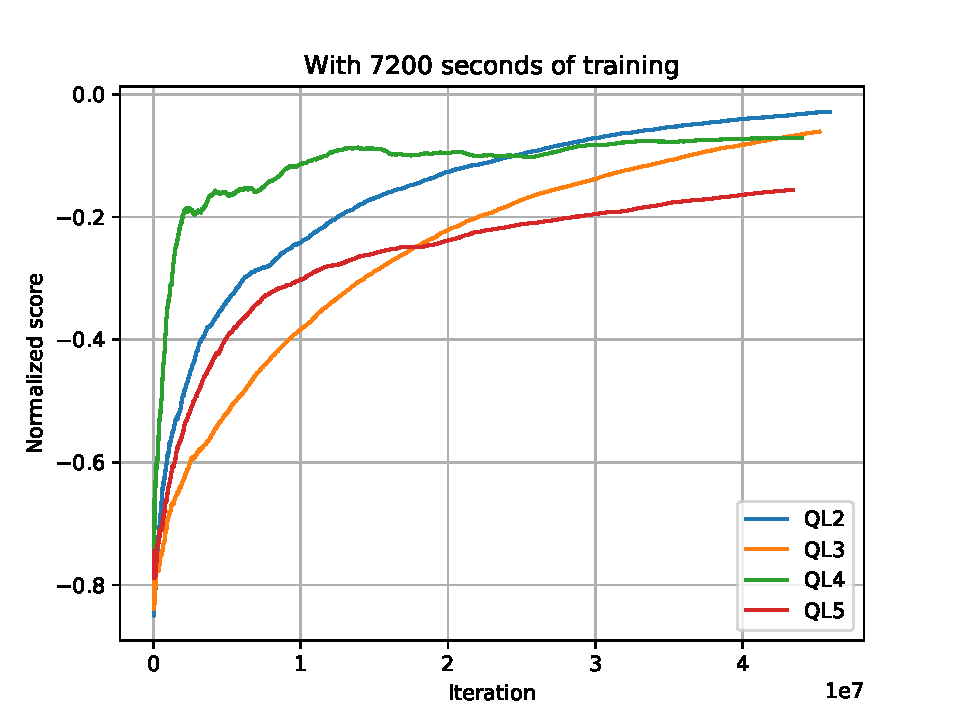
\includegraphics[width=.9\linewidth]{score-7200.pdf}
	\end{center}
\end{frame}


\begin{frame}
\begin{center}
Thanks for your attention.
\end{center}
\vspace{1em}
\begin{thebibliography}{9}

\bibitem{sutton}
R. S. Sutton and A. G. Barto
\textsl{Reinforcement Learning: An Introduction}
{\footnotesize (Very good introduction to RL, draft available online)}

\bibitem{deepmind}
V. Mnih, K. Kavukcuoglu, D. Silver et al.
\textsl{Human-level control through deep reinforcement learning}
Nature 2015 -- 10.1038/nature14236
{\footnotesize (Other Atari games)}

\end{thebibliography}

\end{frame}

\end{document}
